%%%%%%%%%%%%%%%%%%%%%%%%%%%%%%%%%%%%%%%%%%%%%%%%%%
% TODO
% 11After finishing with the paper and supplementary, name all figures as they are in the paper and in the supplementary materials
% make the captions in normal size

\documentclass[12pt]{article}
% Increase margin width for todos
\setlength{\marginparwidth}{2cm}
\usepackage{comment}
\usepackage{geometry}
\geometry{a4paper, margin=0.6in}
\usepackage{setspace}
\usepackage{amsmath}
\usepackage[most]{tcolorbox}
\usepackage{pifont}
\usepackage{graphicx}
\usepackage{hyperref}
\usepackage{capt-of}
\usepackage{caption}
\usepackage{soul}           % For text highlighting
\usepackage{xcolor}         % For color definitions
\usepackage{todonotes}      % For margin notes
\usepackage{enumitem,amssymb}
\usepackage{bm}% bold math
\usepackage{enumitem}


% Define custom colors
\definecolor{softtodogreen}{HTML}{90EE90}  % Light green
\setuptodonotes{color=softtodogreen}

\setstretch{1.5}

% Define different colored highlighting commands
\newcommand{\hlgreen}[1]{\sethlcolor{green!30}\hl{#1}}
\newcommand{\hlred}[1]{\sethlcolor{red!30}\hl{#1}}
\newcommand{\hlyellow}[1]{\sethlcolor{yellow!50}\hl{#1}}
\newcommand{\hlblue}[1]{\sethlcolor{blue!20}\hl{#1}}

% Define custom colors
\definecolor{commentcolor}{RGB}{150, 0, 0}
\definecolor{solved_commentcolor}{RGB}{0, 150, 0}
\definecolor{responsecolor}{RGB}{0, 90, 150}


\newcounter{reviewpoint}
\setcounter{reviewpoint}{0}

% For the numbered reviewer points
\newcommand{\reviewpoint}{%
  \stepcounter{reviewpoint}%
  \vspace{0.5em}%
  {\noindent\textbf{\thereviewpoint.}}%
  \vspace{-1.2em}% Adjust this value to control spacing between number and box
}

% Define custom environments with proper alignment
\newenvironment{reviewercomment}
    {\begin{tcolorbox}[width=\linewidth,colback=gray!5,colframe=commentcolor!50,title=Reviewer Comment,left=5pt,right=5pt]}
    {\end{tcolorbox}}

\newenvironment{solved_reviewercomment}
    {\begin{tcolorbox}[width=\linewidth,colback=gray!5,colframe=solved_commentcolor!50,title=Reviewer Comment,left=5pt,right=5pt]}
    {\end{tcolorbox}}
    
\newenvironment{ourresponse}
    {\begin{tcolorbox}[width=\linewidth,breakable,enhanced,colback=gray!5,colframe=responsecolor!50,title=Response,left=5pt,right=5pt]}
    {\end{tcolorbox}}


% For todos, clean definition without duplicates
\newlist{todolist}{itemize}{2}
\setlist[todolist]{label=$\square$}



\begin{document}

\begin{itemize}

\item[\rlap{\raisebox{0.3ex}{\hspace{0.4ex}\scriptsize \ding{51}}}$\square$]
Coherent spot size simulation: achieve more stastics and try to solve it
\item[\rlap{\raisebox{0.3ex}{\hspace{0.4ex}\scriptsize \ding{51}}}$\square$]
\st{Analytic} dependence on M (covariance estimator + rank of object) 

\item[\rlap{\raisebox{0.3ex}{\hspace{0.4ex}\scriptsize \ding{51}}}$\square$]
Phase retrieval: (a) number of iterations (show plateau) (b) noise + number of realizations (needs good approximation of AC)
\item[\rlap{\raisebox{0.3ex}{\hspace{0.4ex}\scriptsize \ding{51}}}$\square$]
Show convergence graph in some measurements + heatmap of iterations as function of M / function of sparsity
\item[$\square$]
Modify [Kang et al., Nat. Commun., 2023] and if possible try and simulate such solution

\item[$\square$]
Mosaicing experiment

\item[$\square$]
SVD and show depndence of singular vector and energy conservation

\item[$\square$]
Figure of different multiplicative factors and their dependence + Explain more the multiplication of different constants 

\item[\rlap{\raisebox{0.3ex}{\hspace{0.4ex}\scriptsize \ding{51}}}$\square$]
Heatmap of sparsity and M with noise
\item[\rlap{\raisebox{0.3ex}{\hspace{0.4ex}\scriptsize \ding{51}}}$\square$]
Heatmap of sparsity and M

\end{itemize}
\newpage
\title{Response to Reviewers}


\section{Reviewer \#1 Comments (from PDF):}

In this work, the authors extend the matrix approach of optical imaging they have been developing with other groups for the last few years to the context of dynamic scattering media. This topic is of great interest because matrix imaging has shown its great potential for overcoming multiple scattering in the long-standing quest towards deep imaging of complex media such as biological tissues. However, it relies by essence on the hypothesis of a static medium. Their approach relies on the fact that, under the isoplanatic hypothesis, dynamic scattering is mathematically analogous to dynamic illumination in static scattering media. From this analogy, they are then able to use the methods developed in previous papers [13] for scattering compensation under dynamic illumination in which the covariance matrix of the reflected wave-field was investigated rather than just the reflection matrix itself. This covariance matrix has already been recently leveraged to extend the scope of matrix imaging to incoherent (fluorescent) imaging by the authors themselves [14]. This paper is a new important demonstration of the versatility and the universality of matrix approaches to wave imaging in complex media. For incoherent imaging, the demonstration of the superiority of matrix imaging with respect to speckle correlation techniques [28,29] is convincing and might have deserved more publicity than just a short section in the Supplementary Material. For coherent imaging applications, the hypothesis of a constant incident wave-field is a bit contradictory with the problem of dynamic scattering and would deserve more discussion.  

As often with this group, this work is technically of excellent quality and its presentation is elegant. The experiments based on rotating diffusers are rather simple and allow the authors to illustrate nicely the concept. However, one can wonder whether the idea proposed by the authors can go beyond imaging through a thin dynamic diffusive layer and to which extent it can be applied to real 3D imaging situations like for biomedical or LiDAR applications. I detail below the main points that, in my opinion, would deserve more discussion before publication.

\begin{ourresponse}
    We thank the Reviewer for their positive evaluation of our work, recognizing its significance in extending matrix-based imaging to dynamic scattering media and its potential impact.
\end{ourresponse}

\begin{enumerate}[label=\arabic*.]
\item \leavevmode
\end{enumerate}
\vspace{-1em}
\begin{solved_reviewercomment}
    For instance, in the coherent imag ing experiment depicted in Fig.~\ref{fig_5}, the approach requires a constant incident wave-field, which is complicated if one wants to image through a dynamic scattering medium. In the present experiment, the authors circumvent this issue by focusing the incident wave-field in the diffuser plane such that the beam waist is contained in one coherence length of the diffuser. However, in practical situations, the scattering medium is three-dimensional, and the condition of a constant incident wave-field becomes impossible to fulfill. In real life, dynamic scattering impacts both the incident and reflected wave-fields. The authors do not discuss really this apparent contradiction between the assumption of a constant incident wave-field and dynamic scattering that will break this invariance.
\end{solved_reviewercomment}

\begin{ourresponse}
    We appreciate the reviewer's observation about the apparent contradiction between dynamic scattering and our requirement for constant illumination in the coherent imaging experiment (Fig.~\ref{fig_5}). 
    
    In our coherent demonstration, we circumvented this challenge by focusing the illumination beam onto a small area of the diffuser (smaller than its correlation length), effectively sampling only a single "phase patch" as the diffuser rotates. However, we recognize this approach is not feasible for volumetric scattering media where maintaining constant illumination becomes challenging.
    
    To address this limitation transparently in our manuscript, we have added the following clarification to the Discussion section:
    
    \begin{quote}
        "Additionally, we note that for coherent imaging through dynamic scattering, our current approach is limited to scenarios where effectively constant illumination can be maintained at the object plane. While demonstrated here with a thin diffuser, volumetric scattering presents additional challenges that require further development."
    \end{quote}
    
    Beyond this manuscript revision, we propose a hybrid approach that could extend our method to volumetric dynamic media without requiring focused illumination:
    \begin{enumerate}
        \item For each realization of the dynamic scatterer, rapidly acquire multiple ($K \gg 1$) holograms under different speckle illuminations (created with an additional diffuser in the illumination path)
        \item Use coherence gating on each individual hologram to determine the correct object depth and eliminate unwanted reflections
        \item Incoherently sum the intensity patterns to create "macro-frames": $I_m(x,y,z=z_{obj}) = \sum_{k=1}^{K}|E_{m,k}(x,y,z=z_{obj})|^2$ 
        \item Process these macro-frames using I-CLASS as in our incoherent experiments
    \end{enumerate}
    
    This protocol creates effectively uniform illumination through incoherent summing (as in the incoherent experiment with the rapidly rotating diffuser in the illumination path) while preserving the depth-selectivity and reflection-filtering advantages of coherent light. Each resulting macro-frame follows $I_m = P_m * O$, making the problem mathematically equivalent to our incoherent imaging scenario.
    
    Our current experimental demonstration served as a controlled environment to validate the fundamental principles of our approach. The hybrid method described above offers a promising path forward for complex volumetric media while maintaining the benefits of coherent imaging. Additionally, we highlight the applicability of our approach to advanced systems such as flexible multi-core fiber endoscopes (as demonstrated by Choi et al. [Flexible-type ultrathin holographic endoscope for microscopic imaging of unstained biological tissues]), where uniform illumination via single-mode excitation can be straightforwardly achieved.
\end{ourresponse}


\begin{enumerate}[label=\arabic*., resume]
\item \leavevmode
\end{enumerate}
\vspace{-1em}
\begin{solved_reviewercomment}
    Another issue of three-dimensional scattering is that it breaks the isoplanatic assumption on which the current approach relies. The authors mention in the discussion the idea of mosaicking the field-of-view but it somehow requires a roughly focused incident wave-field and only applies to moderate scattering. Another route is a multi-conjugate adaptive optics scheme in which multiple scattering trajectories are rectified by compensating aberrations from a stack of phase screens conjugated with different planes inside the scattering medium [Kang et al., Nat. Commun., 2023]. Would the current approach proposed by the authors be compatible with such a multi-conjugate strategy? It might be relevant to discuss this point in the conclusion.
\end{solved_reviewercomment}

\begin{ourresponse}
    We thank the reviewer for highlighting this important limitation. We have demonstrated reconstruction through a thin scattering dynamic layer in our current work. The extension to thick scattering media represents an important challenge and direction for future research.

    In conventional CLASS or computational wavefront shaping, thick scatterers can be addressed by using multi-conjugate approaches with multi-layer scattering profiles. However, our approach presents a unique twist: in our formulation, the dynamic medium plays the role that would normally be occupied by the object in conventional CLASS implementations. This role reversal creates both challenges and opportunities.
    
    The modeling and treatment of thick targets proposed in the recent work by Park et al. \cite{oh2025digital} may offer a pathway forward. In that work, the authors developed techniques for handling thick objects rather than treating them as purely planar. Since in our case the dynamic medium mathematically functions as the "object," adapting these techniques could potentially allow us to extend our approach to volumetric scattering media.

    Additionally, another potential approach could be derived from the gradient-descent model-based algorithm recently developed by Haim et al. in their computational holographic wavefront shaping work \cite{haim2025image}. This method's flexibility in computational wavefront correction might offer alternative strategies for handling thick scattering media.
    
    We have added the following paragraph to the discussion section:
    \begin{quote}
        "While we have focused our proof-of-principle demonstrations on isoplanatic scattering conditions, extending our approach to thick dynamic scattering media remains an important challenge. Recent advances in modeling thick targets rather than planar ones, such as those presented by Park et al. \cite{oh2025digital}, suggest potential pathways for adaptation to our scenario, where the dynamic medium mathematically plays the role of the object. Future work could explore combining our approach with multi-conjugate modeling, treating thick media as a series of thin scattering layers at different depths, each contributing its own phase and amplitude distortions to the overall scattering process."
    \end{quote}
    
\end{ourresponse}

\begin{enumerate}[label=\arabic*., resume]
\item \leavevmode
\end{enumerate}
\vspace{-1em}
\begin{solved_reviewercomment}
    One last point which is not really discussed in the paper is the number of required independent frames \(M\) to converge towards a reliable estimation of the object or, in other words, the scaling of the estimator bias with respect to this number \(M\). An analytical formulation of the problem could be performed to derive this number, which is important for future implementations of the method. I guess this number will depend on the object complexity/sparsity.
\end{solved_reviewercomment}
    
\begin{ourresponse}
    We appreciate the reviewer's important question about the number of required independent frames for reliable estimation. To address this systematically, we conducted a set of numerical simulations investigating the relationship between reconstruction quality, number of realizations (M), and object sparsity. 

    The theoretical foundation of CTR-CLASS, as established in previous work by Lee et al., indicates a logarithmic dependence of the required number of measurements on the degrees of freedom (i.e., the number of camera pixels $N$). However, this theoretical scaling is modified in practice by additional factors, including object complexity (sparsity) and signal-to-noise ratio (SNR). These factors play crucial roles in determining the practical minimum number of frames needed for successful reconstruction.

    We have added a new supplementary section ("Dependence of Reconstruction Quality on Number of Realizations and Object Sparsity") that addresses this question.
    
    % \hlred{Take from I-CLASS / Acusto-optic the paragraph about the theoretical dependence on M which is logarithmic (from the CTR paper) and add that there are additional factors to this theory such as the object complexity and SNR}.
    
    \begin{quote}
        \section*{Dependence of Reconstruction Quality on Number of Realizations and Object Sparsity}

        % \hlred{I suggest inserting something about how statistical siginficant is this result? how many experiments are in each heatmap cell? and what is the std between expereimnts (you have 3 random variables, the random object, the shot noise and the PSFs, maybe freeze 2 each time and run it to understand if they have the same effect}.

        
        To study the dependence of the reconstruction quality on the number of realizations and object complexity (sparsity), we numerically simulate the reconstructions at a varying number of random realizations (M) for different object complexities (sparsity) for incoherent and coherent imaging modalities.
        The results of the simulation for varying SNR values at an object sparsity are given in Figure Fig.~\ref{fig_S8}
        To ensure statistical robustness, each data point in these heatmaps represents the average outcome from 10 independent numerical experiments.

        
        \begin{minipage}{\linewidth}
            \centering
            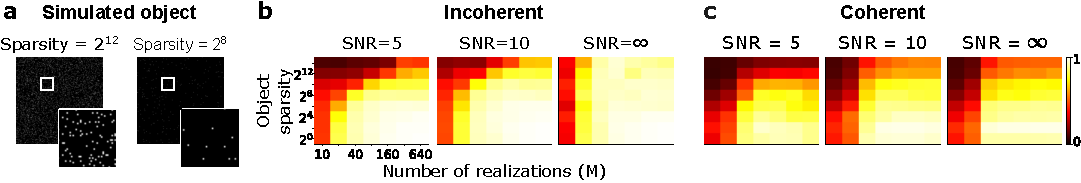
\includegraphics[width=0.93\textwidth]{figures/figure_S8.pdf}
            \renewcommand{\thefigure}{S8}
            \captionof{figure}{\footnotesize \textbf{ Reconstruction fidelity as a function of number of realizations and object sparsity.} 
            Cross-correlation scores between reconstructed and ground truth images are shown as heatmaps for different imaging scenarios. \textbf{a} Example simulated objects with different sparsity levels: $2^{12}$ (left) and $2^8$ (right) bright points. \textbf{b} Incoherent imaging results under different SNR conditions: SNR=5 (left), SNR=10 (middle), and SNR=$\infty$ (right). \textbf{c} Coherent imaging results under the same SNR conditions: SNR=5 (left), SNR=10 (middle), and SNR=$\infty$ (right). The horizontal axis shows the number of realizations (M), and the vertical axis shows object sparsity (represented as the number of bright points). Color scale indicates correlation coefficient from 0 to 1. Each data point represents the average result from 10 distinct numerical experiments with different random objects under identical parameters. For all simulations, a camera pixel count of N=350$^2$ was used.}
            \label{fig_S8}
        \end{minipage}

        These results demonstrate that sparser objects can be reconstructed with fewer realizations, while complex objects need substantially more measurements. Higher SNR conditions predictably improve reconstruction quality, and coherent imaging appears to require more measurements than incoherent imaging for equivalent fidelity.

                   
    \end{quote}
    
\end{ourresponse}



\textbf{More Specific Comments:}


\begin{enumerate}[label=\arabic*., resume]
\item \leavevmode
\end{enumerate}
\vspace{-1em}
\begin{solved_reviewercomment}
    The supplementary Section S2 that shows the impact of correlations between speckle patterns is very interesting and might have deserved a place in the main manuscript. In this Supplementary Section, these correlations arise from energy conservation (phase-distortions). Maybe a singular value (or equivalently eigenvalue) decomposition of the covariance matrix \cite{badon2020distortion}(citation [10] in manuscript) can help in that case? The first singular vector would be less affected by these negative correlations than the CLASS algorithm. Can the authors comment on that? 
\end{solved_reviewercomment}

\begin{ourresponse}
    \begin{comment}
        \hlred{But citation [10]  doesn't perform SVD on the covariance matrix: A. it is not on the covariance but on the full matrix, and B. it is also not on the matrix but on the 'de-scanned' / 'distortion' matrix, which is different. This cannot apply here where the energy conservation creates a problem in the covariance calculation, **before applying algorithm**}

        \hlred{Maybe refer to Wonshik's work on SVD (the Science Adavnces one https://www.science.org/doi/10.1126/sciadv.abo4366) and show him the effect of pre-processing the measurement matrix with SVD filtering, create a graph where the x axis is the number of non-zero singular values, and the correlation to GT, and see if there is a value smaller than M that will give better correlation}
    \end{comment}
    

    We thank the reviewer for this insightful comment. Following this recommendation, we have added the following discussion to the main manuscript:
    
    \begin{quote}
        Our analysis revealed that energy conservation in phase-only speckle patterns introduces troublesome spatial correlations that can cause background haze in the reconstructions. We addressed this by simply applying varying intensity scaling across frames during post-processing. It would be interesting to study whether a singular value decomposition filtering (SVD) of the measurement matrix or the distortion matrix \cite{badon2020distortion,jo2022through} can help to address these effects.
        
        % It was recently shown that SVD-based filtering of the distortion matrix \cite{badon2020distortion} or the reflection matrix \cite{jo2022through} can XXXXX. An in-depth study of the potential of advnaced filtering of the measurement or covariance matrix will be the focus of future work.

        It was recently shown that SVD-based filtering of the distortion matrix \cite{badon2020distortion} or the reflection matrix \cite{jo2022through} can help isolate single-scattering contributions from complex systems with multiple scattering. In the distortion matrix approach \cite{badon2020distortion}, the first singular vectors capture the most XXXX signal contributions, while in \cite{jo2022through}, they showed that eigenvalue decomposition of a time-gated reflection matrix can effectively attenuate uncorrelated multiple scattering while retaining single-scattering signals with strong wave correlation. An in-depth study of the potential of advanced filtering of the measurement or covariance matrix will be the focus of future work.

        
        The full analysis of the effects of the energy-conservation originated correlations on the reconstruction, and our approach for mitigating them, is detailed in Supplementary Section S2 and Supplementary Figure S3.
    \end{quote}
    
    We maintained the detailed analysis in Supplementary Section S2 as you suggested, while bringing the key insight to readers' attention in the main text.

\end{ourresponse}


    
\begin{enumerate}[label=\arabic*., resume]
\item \leavevmode
\end{enumerate}
\vspace{-1em}
\begin{solved_reviewercomment}
    The authors show how to circumvent this issue by a multiplication of each frame by a fixed scalar value. This is interesting, but the choice of the multiplication factor from one to two lacks justification. Can the authors provide more details about this choice? 
\end{solved_reviewercomment}

\begin{ourresponse}
We thank the reviewer for this question about our choice of multiplication factors. To address this, we conducted a systematic study examining how different modulation depths affect reconstruction quality.

We have added a new section to the Supplementary Materials titled "Effect of Modulation Depth on Reconstruction Quality" that demonstrates this trade-off. Here is the full section:

\begin{quote}
\section*{Effect of Modulation Depth on Reconstruction Quality}

As discussed in Supplementary Section S2, energy conservation introduces off-diagonal correlations in the covariance matrix that can degrade reconstruction quality. We addressed this by applying variable intensity scaling across the captured frames, with multiplication factors linearly varying from 1 to 2 across frames.

To investigate the optimal range for this modulation, we conducted a study examining how different modulation depths affect reconstruction quality. For each depth value, we applied a linear scaling to our experimental data where the multiplication factor for the $m$-th frame (out of $M$ total frames) was:

\begin{equation}
    f_m = 1 + \frac{m-1}{M-1} \cdot (\alpha -1) = 1, 2, 3, ..., \alpha
\end{equation}

where $\alpha$ controls the total range of modulation with corresponding modulation depth $\frac{\alpha-1}{\alpha+1}$.

\begin{comment}
    We can rewrite this equation directly in terms of the modulation depth $d$ by solving for $\alpha$:

    \begin{align}
    d &= \frac{\alpha-1}{\alpha+1} \\
    d(\alpha+1) &= \alpha-1 \\
    d\alpha + d &= \alpha - 1 \\
    d\alpha - \alpha &= -1 - d \\
    \alpha(d-1) &= -1 - d \\
    \alpha &= \frac{-1-d}{d-1} = \frac{1+d}{1-d}
    \end{align}

    Substituting this into our original equation:
    
    \begin{align}
    f_m &= 1 + \frac{m-1}{M-1} \cdot \left(\frac{1+d}{1-d} - 1\right) \\
    &= 1 + \frac{m-1}{M-1} \cdot \frac{1+d-(1-d)}{1-d} \\
    &= 1 + \frac{m-1}{M-1} \cdot \frac{2d}{1-d}
    \end{align}
    
    Therefore, the multiplication factor for the $m$-th frame in terms of modulation depth $d$ is:
    
    \begin{equation}
        f_m = 1 + \frac{m-1}{M-1} \cdot \frac{2d}{1-d}
    \end{equation}
\end{comment}


\begin{minipage}{\linewidth}
    \centering
    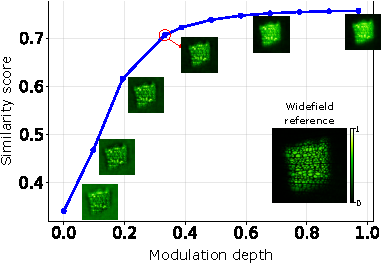
\includegraphics[width=0.93\textwidth]{figures/Figure_S9.pdf}
    \renewcommand{\thefigure}{S9}
    \captionof{figure}{\footnotesize \textbf{Effect of modulation depth on reconstruction quality.} The similarity score (y-axis) shows the Pearson correlation coefficient between the reconstructed and ground-truth images as modulation depth increases. Example reconstructions demonstrate the progressive elimination of background haze as modulation increases, while at higher modulation depths, some haze begins to appear within the object itself. The red circle indicates our chosen modulation depth, which offers a good trade-off in this balance.}
    \label{fig_S9}
\end{minipage}
%\hlred{Explain  what is the similarity score in the caption, change y-label to correlation, write in the caption 'Pearson correlation'}

% \hlred{Add $\alpha$ to x label}


Our results show that without adding a modulation (modulation depth = 0), the reconstructions display a significant background haze. As modulation increases, this background haze diminishes progressively. However, at very high modulation depths, while the background continues to reduce, the contrast is somewhat lowered, which may be the result of an imperfect estimation of the MTF in the I-CLASS algorithm.  Modulation depths of 0.3-0.5 used in our main experiments provide an effective trade-off between these competing effects. 
Additional improvements of this point can will be the focus of future work.

%\hlred{Maybe show the $PP^T$ for different $\alpha$-s}


\end{quote}
\end{ourresponse}


    
\begin{enumerate}[label=\arabic*., resume]
\item \leavevmode
\end{enumerate}
\vspace{-1em}
\begin{solved_reviewercomment}
    Even if the I-CLASS and CTR-CLASS have already been presented in previous papers, I would suggest describing them in the Methods section to make the paper self-sufficient. 
\end{solved_reviewercomment}

\begin{comment}
    \hlred{\textbf{Elad's comment:}            
    The descriptions in the methods part are not clear without the matrix description, and the MTF deconvolution part is not relevant here, it should be totally rephrased and organized, and in the supplementary it is also very long and most parts are not relevant to this paper, you don't have to derive all the CLASS algorithm again, I would just write something like $I=P*(O\cdot E_{in}*P_{in})$ and therefore $R=POP$ and CLASS is a matrix unitary decomposition algorithm, after that in few lines about CTR and just bring the final memory efficient term of each phase correction iteration, (maybe write in algorithm pattern as shown in CS papers) And write that the MTF estimation is just like speckle correlation methods. You can take my AO paper as reference, I explained there more briefly}
\end{comment}

\begin{comment}
    **From Gil:**
    We employ the I-CLASS algorithm \cite{ weinberg2024noninvasive}, which is based on the CLASS algorithm \cite{kang17, kang2024implementation}, which corrects incident and reflected aberrations within an isoplanatic patch. Under the assumptions of isoplanatism and a thin planar object, the problem simplifies to estimating three rank-1 vectors: the incident aberration, the reflected aberration, and the thin planar object. In the specific case of CTR-CLASS, this further simplifies the estimation to two rank-1 vectors, as the incident and reflected aberrations are identical. CTR-CLASS is based on covariance analysis of random speckle illuminations, analogous to the retrieval of Green’s functions in passive correlation imaging [Maybe cite Wapenaar, Phys. Rev. Lett. 93, 254301 (2004)?], enabling a compressed estimation of the reflection matrix. As mentioned, we use dynamic scattering to replace the role of the random speckle illuminations, but as the covariance matrix of a set of camera frames of a rapidly varying dynamic scattering sample has the same mathematical form as a reflection matrix of a static medium, the same algorithm can be applied in this use case. We note that the addition of the $\vec{k}$-space amplitude correction, as demonstrated in the I-CLASS paper \cite{weinberg2024noninvasive}, is required for both the incoherent and coherent imaging cases, as in stellar speckle interferometry \cite{labeyrie1970attainment}.

    In the specific context of this paper... (add something similar to the \subsubsection*{Memory-efficient CLASS iterations}, but swap the roles of P and O - write the algo iterations)
\end{comment}

\begin{ourresponse}
We thank the reviewer for this suggestion.

We have added a comprehensive description of the I-CLASS algorithm to the Methods section as suggested.
\begin{quote}
    \subsection*{I-CLASS algorithm for dynamic scattering compensation}
        We employ the I-CLASS algorithm \cite{weinberg2024noninvasive}, an extension of the CLASS algorithm \cite{kang17, kang2024implementation} designed to correct incident and reflected aberrations within an isoplanatic patch. The CLASS algorithm decomposes the reflection matrix to separate the object from scattering distortions, while CTR-CLASS and I-CLASS apply the same decomposition principles to the covariance matrix. Under the assumptions of isoplanatism and a thin planar object, the problem simplifies to estimating three rank-1 vectors: the incident aberration, the reflected aberration, and the thin planar object. In the specific case of CTR-CLASS, this further simplifies the estimation to two rank-1 vectors, as the incident and reflected aberrations are identical. CTR-CLASS is based on covariance analysis of random speckle illuminations, similar to the retrieval of Green's functions in passive correlation imaging \cite{wapenaar2004retrieving}, which enables a compressed estimation of the reflection matrix.
        
        In our dynamic scattering scenario, the key insight is the mathematical role exchange between the object and PSF compared to the standard CTR-CLASS framework. We arrange the captured camera frames as columns of a measurement matrix $\textbf{A}$, where each column represents one image realization. In conventional CTR-CLASS / I-CLASS (with static scattering), each recorded frame follows the convolution equation $I_m(\vec{r}) = P(\vec{r}) \ast O_m(\vec{r})$ with a static PSF and varying illuminated objects, which can be expressed in matrix form as $\textbf{A} = \textbf{P}\textbf{O}\textbf{S}$. In our dynamic scattering approach, the equation becomes $I_m(\vec{r}) = P_m(\vec{r}) \ast O(\vec{r})$, which due to convolution commutativity can be rewritten as $I_m(\vec{r}) = O(\vec{r}) \ast P_m(\vec{r})$. This is represented in matrix form as $\textbf{A} = \textbf{O}\textbf{P}$, where $\textbf{O}$ is now a Toeplitz convolution matrix with the object function as the convolution kernel, and $\textbf{P}$ contains the different PSF realizations as its columns.

        This mathematical duality allows us to apply the same algorithm to reconstruct the object instead of the scattering medium without modifying the core algorithm structure. Weinberg et al. \cite{weinberg2024noninvasive} enhanced the basic approach with both a memory-efficient implementation and amplitude correction, addressing not only phase but also amplitude distortions caused by scattering. The algorithm operates in the Fourier domain, where convolution becomes multiplication, making the decomposition more tractable. 
        
        For each iteration $t = 1...T$, the algorithm computes a correction vector:
        \begin{eqnarray}
            \vec{z}_{t+1}=\sum_{q=1}^{M}(\tilde{\textbf{A}}_t^* \odot ((\tilde{\textbf{A}}_t^{(ud)^*}*\tilde{\textbf{A}}_t^{(lr)})_{:,M-1} \star \tilde{\textbf{A}}_t^{(ud)}))_{:,q}
        \end{eqnarray}
        
        The matrix is then updated through phase correction in the Fourier domain:
        \begin{eqnarray}
            \tilde{\textbf{A}}_{t+1}=diag\{e^{i\frac{\vec{z}_t}{|\vec{z}_t|}}\}\tilde{\textbf{A}}_t
        \end{eqnarray}
        
        Here, $\tilde{\textbf{A}}$ denotes the 2D Fourier transform of the mean-subtracted measurement matrix, $\tilde{\textbf{A}}^{(ud)}$ is $\tilde{\textbf{A}}$ with each column flipped upside-down, and $\tilde{\textbf{A}}^{(lr)}$ is $\tilde{\textbf{A}}$ with rows flipped left-to-right. The symbols $\odot$, $*$, and $\star$ represent element-wise multiplication (Hadamard product), 2D convolution, and 2D correlation operators, respectively. The complex conjugate of a matrix is denoted by the superscript $*$, and $\textbf{X}_{:,q}$ represents the $q$-th column of matrix $\textbf{X}$.
        
        This approach enables reconstruction of complex objects through dynamic scattering media using only a small number of measurements (M=150 in our experiments), making it practical for imaging scenarios where rapidly varying scattering would otherwise prevent clear visualization.
\end{quote}

\end{ourresponse}


\begin{enumerate}[label=\arabic*., resume]
\item \leavevmode
\end{enumerate}
\vspace{-1em}
\begin{solved_reviewercomment}
    The same remark holds for the Fresnel operators applied at different stages of the post-processing for the holographic experiment.
\end{solved_reviewercomment}

\begin{ourresponse}
    We thank the reviewer for this helpful suggestion. The revised manuscript now includes a detailed description of the Fresnel propagation operator used in the holographic reconstruction. This has been added to the \textbf{Methods} section titled "Fresnel Propagation via Fourier-Domain Transfer Function".
    \begin{quote}
        \subsection*{Fresnel Propagation via Fourier-Domain Transfer Function}
        \label{Fresnel_propagation}
        In Fig.~\ref{fig_5}, we present the object field located at the physical object plane, $z_{\text{obj}}$. However, since we measure the field on the diffuser plane, the I-CLASS algorithm reconstructs the complex field in the plane of the scattering layer, denoted as $E_o(x, y, z_{\text{scatt}})$. To visualize the field at the object plane, we propagate the reconstructed field from the diffuser plane to the object plane using Fresnel propagation under the paraxial approximation.
        
        This propagation is efficiently implemented in the Fourier domain using the Fresnel transfer function:
        
        \begin{equation}
            E_o(x, y, z_{\text{obj}}) = \mathcal{F}^{-1} \left\{ \tilde{E}_o(f_x, f_y, z_{\text{scatt}}) \cdot H(f_x, f_y; \Delta z) \right\}
        \end{equation}
        
        where:
        - $ \tilde{E}_o(f_x, f_y, z_{\text{scatt}}) = \mathcal{F}\{ E_o(x, y, z_{\text{scatt}}) \} $ is the 2D Fourier transform of the reconstructed field,
        - $ H(f_x, f_y; \Delta z) $ is the Fresnel transfer function,
        - $ \Delta z = z_{\text{obj}} - z_{\text{scatt}} $ is the propagation distance,
        - $ \mathcal{F} $ and $ \mathcal{F}^{-1} $ denote the 2D Fourier and inverse Fourier transforms.
        
        The Fresnel transfer function in terms of spatial frequency is:
        
        \begin{equation}
            H(f_x, f_y; \Delta z) = \exp\left[ i \frac{2\pi \Delta z}{\lambda} \right] \cdot \exp\left[ -i \pi \lambda \Delta z (f_x^2 + f_y^2) \right]
        \end{equation}
        
        Here:
        - $ \lambda $ is the illumination wavelength,
        - $ (f_x, f_y) $ are the spatial frequency coordinates corresponding to the real-space axes $ (x, y) $.
        
        This formulation supports forward and backward propagation by simply changing the sign of $ \Delta z $, and is especially suitable for numerical implementation via Fast Fourier Transforms.
        
    \end{quote}

            
\end{ourresponse}


    
\begin{enumerate}[label=\arabic*., resume]
\item \leavevmode
\end{enumerate}
\vspace{-1em}
\begin{solved_reviewercomment}
    In that respect, it is not really clear to me why, in the holographic experiment, the I-CLASS reconstructed object field is obtained in the scattering layer plane? A more detailed description of the method is needed.
\end{solved_reviewercomment}

\begin{ourresponse}
    \begin{comment}
    \hlred{I would add that we measure on the diffuser plane and hence the multiplicative factor is with the propagated object, so that is the object that is reconstructed}


    \hlred{Write equations... original CLASS $POP\quad \overrightarrow{}\tilde{P}\tilde{O}\tilde{P}$, Here $O_{prop}PO_{prop}$ where $O_{prop}$ is diagonal and $P$ is the envelope, no Fourier needed}
    \end{comment}

    We thank the reviewer for bringing this important point to our attention.
    
    This decision follows the principle of conjugation in adaptive optics. Conjugate correction involves placing the corrective elements (or, in computational approaches, applying corrections) in a plane optically conjugated to the primary source of aberrations. By measuring and applying corrections at the plane where phase (and potentially also amplitude) multiplicative distortions occur (the thin scattering layer plane), we achieve more efficient correction across the field of view. This concept is well established in the literature, such as in the works by Mertz et al. \cite{mertz2015field}, Kwon et al. \cite{kwon2023computational}, and Sunray et al. \cite{sunray2024beyond}.
    
    In the standard case, the CLASS/I-CLASS algorithm finds the phase distortion at this exact plane where the distortions can be described as multiplicative distortions, i.e., the scattering layer transmission-matrix is a diagonal matrix, i.e., can be effectively considered as a thin phase (and in I-CLASS also amplitude) mask. Mathematically, this can be represented as $E_{meas zdiff}(r)=O_{prop}(r)e^{i\phi_{scatt}(r)}$, where $O_{prop}(r)$ is the propagated object field and $e^{i\phi_{scatt}(r)}$ represents the phase distortion at the scattering layer. The output of the CLASS algorithm in the standard case, where the scattering medium is static and the target is dynamically illuminated, is thus the correction phase mask at the scattering layer plane. 

    In our case, the scattering medium and the target change roles: the scattering function changes throughout the measurements while the object remains fixed. Running the I-CLASS algorithm on our dataset thus results in an output that is the object phase and amplitude function at the scattering layer plane. This complex-valued field is then back-propagated to any desired distance until a sharp, focused image of the target is obtained (see the new Supplementary Fig.~\ref{fig_S6}).

    \begin{comment}
        \begin{tcolorbox}[enhanced, colback=gray!5, colframe=black!50!blue, title=Mathematical Explanation]
    From a mathematical perspective, measuring at the diffuser plane provides a natural structure for applying CLASS-based algorithms. In the diffuser plane, our measurement matrix $A$ can be expressed as:
    
    $A = OP$

    

    where $O$ is a diagonal matrix containing the propagated object field, and $P$ is a matrix whose columns represent the different diffuser realizations (which are uncorrelated due to the rotation between acquisitions).
    
    The covariance matrix we compute from these measurements is:
    $$AA^\dagger = OPP^\dagger O^\dagger = O|P|^2O^\dagger$$
    
    For uncorrelated columns in $P$, we will have $|P|^2$ as a diagonal matrix. This mathematical structure directly matches the form expected by CLASS algorithms:
    \begin{itemize}
        \item In conventional CLASS, the input has the form $POP^\dagger$, where $P$ is a convolution (Toeplitz) matrix and $O$ is diagonal
        \item In our case, with the roles of object and scattering medium effectively reversed, we have $O|P|^2O^\dagger$, where here $O$ is a convolution (Toeplitz) matrix and $P$ is diagonal
    \end{itemize}
    
    By measuring at the diffuser plane, we naturally obtain this required matrix structure without additional transformations, making this choice mathematically convenient.
    \end{tcolorbox}
    \end{comment}
\end{ourresponse}



\textbf{Typos:}

\begin{enumerate}[label=\arabic*., resume]
\item \leavevmode
\end{enumerate}
\vspace{-1em}
\begin{solved_reviewercomment}
    Page 2: “Thus, enabling a straightforward fully interpretable extension of matrix-based methods to rapidly dynamic scatterers, reconstructing complex megapixel-scale images through rapidly varying scattering. Importantly…” This is not a sentence, please rephrase.
\end{solved_reviewercomment}

\begin{ourresponse}
    We appreciate the reviewer’s comment and have revised it in the updated manuscript. The revised version now reads:
    
    \begin{quote}
        Thus, our approach provides a natural and fully interpretable extension of matrix-based imaging techniques to the case of rapidly dynamic scatterers. It enables the reconstruction of complex, megapixel-scale images through strongly time-varying scattering. Importantly, unlike state-of-the-art neural-networks-based techniques, our approach does not require assuming a slowly varying medium, making it suitable for dynamic scattering.
    \end{quote}
    
\end{ourresponse}



\begin{enumerate}[label=\arabic*., resume]
\item \leavevmode
\end{enumerate}
\vspace{-1em}
\begin{solved_reviewercomment}
    Page 7: “These experiments’ experimental setup…” Please rephrase.
\end{solved_reviewercomment}

\begin{ourresponse}
    We have revised the sentence to read: "The experimental setup and results for these experiments..." which removes the redundancy and improves clarity.
\end{ourresponse}


\newpage

\section{Reviewer \#2 Comments (from email):}

In this manuscript the authors propose to use the I-CLASS algorithm (which was developed in the same group) to deconvolve the unknown object from the (many) unknown point spread function measured through a dynamic scattering medium. This builds on a previous paper from the same group (ref 14, as far as I can see still unpublished).

\textbf{Does the approach works?} Yes, the results in Fig. 2 alone are convincing enough.

\textbf{Are the result novel?} Yes. The algorithm itself is not new, but its application is.

\textbf{Is the paper written in a way such that somebody knowledgeable in optics but not an ultra-specialist in imaging through scattering media will be able to replicate the results and build up on them?} Not really. 

\begin{enumerate}[label=\arabic*.]
\item \leavevmode
\end{enumerate}
\vspace{-1em}
\begin{solved_reviewercomment}
    The main culprit is that the whole CRT-CLASS/I-CLASS are not well-known algorithms, and the only reference given to readers to make themselves familiar with them is not self-contained. \textbf{This has a very easy fix:} add a section in the supplementary information with an explanation of how and why the algorithm works (there is no space restriction there, so there is also no excuse to provide the necessary information).
\end{solved_reviewercomment}
\begin{ourresponse}
    It is the same comment as the first referee.
\end{ourresponse}

\begin{enumerate}[label=\arabic*., resume]
\item \leavevmode
\end{enumerate}
\vspace{-1em}
\begin{solved_reviewercomment}
    Another point that is likely to make the life on a non-specialist unnecessarily hard is that eq. 1 is only valid within the isoplanatic patch. For objects larger than the isoplanatic patch nothing of what is presented here will work. This is only briefly addressed at the end of the Discussion section (largely swiping it under the carpet) but if not tackled at the beginning is likely to confuse people.
    
\end{solved_reviewercomment}

\begin{ourresponse}
    We appreciate the reviewer's concern about the isoplanatic patch limitation. We had already mentioned this constraint in the opening paragraph of the Principle section, highlighting that "all experiments and analysis in this work require the imaged object to be contained within the isoplanatic patch of the scattering medium; for objects larger than this patch, the approach presented here would not directly apply without additional modifications such as field segmentation."

    To further emphasize this point and ensure clarity for non-specialist readers, we have also added an explicit note immediately following Equation 1 reiterating this constraint:
    
    \begin{quote}
        "It is important to note that this convolution model is strictly valid only for objects within an isoplanatic patch. All experiments in this work were designed within this constraint, with potential extensions to larger fields of view or thick complex media, which are discussed in the final section."
    \end{quote}
    
    This addition ensures that readers are aware of this limitation from the outset, helping non-specialists better understand the applicability of our approach without having to wait until the Discussion section.
\end{ourresponse}



A few more minor points:

\begin{enumerate}[label=\arabic*., resume]
\item \leavevmode
\end{enumerate}
\vspace{-1em}
\begin{solved_reviewercomment}
    In the introduction the authors claim that iterative phase retrieval lacks guaranteed convergence, which is technically not true. Convergence might take a VERY long time, but it will eventually happen (see \url{https://doi.org/10.1364/AO.21.002758}).
\end{solved_reviewercomment}
\begin{comment}
    ~\\
   \hlred{I recommend applying phase retrieval for millions of iterations with large M to show convergence graph}             
 \end{comment}

\begin{ourresponse}
    We thank the reviewer for their insight. We have revised the text to more accurately reflect the nature of iterative phase retrieval, acknowledging that convergence is possible, albeit potentially time-consuming. The revised sentence now reads:  
    \begin{quote}
        "However, despite this advantage, these techniques are hindered by their reliance on iterative phase retrieval \cite{fienup1978reconstruction}, which can require extensive computational time to converge."
    \end{quote}
    
\end{ourresponse}



\begin{enumerate}[label=\arabic*., resume]
\item \leavevmode
\end{enumerate}
\vspace{-1em}
\begin{solved_reviewercomment}
    Just below the above statement there are two sentences beginning with "while" which looks like they are the leftover of some copy-paste during editing.
\end{solved_reviewercomment}
\begin{ourresponse}
    We thank the reviewer for their careful reading. We have removed the redundant sentence and simplified the text to improve clarity and flow. The revised text now reads:
    \begin{quote}
        "While deterministic bispectrum reconstruction can address the convergence challenge of phase retrieval, it still requires averaging a large number of speckle grains, limiting the reconstruction to simple objects."
    \end{quote}
\end{ourresponse}
% \hlred{Write something about that it is not really cheating since in incoherent illumination passive constant illumination such as the sun...}

        
\begin{enumerate}[label=\arabic*., resume]
\item \leavevmode
\end{enumerate}
\vspace{-1em}
\begin{solved_reviewercomment}
    The results shown in Fig. 2 and 3, albeit impressive, require the target to be illuminated from behind, which makes this whole approach invasive. I know the author never explicitly claim non-invasiveness, but they also never make this point clear.
\end{solved_reviewercomment}

\begin{ourresponse}
    We thank the reviewer for highlighting this important point.
    We fully agree that the initial results presented in Figures 2 and 3 require illumination from behind the sample, which makes the approach invasive. 
    
    However, it is worth noting that this illumination geometry is not fundamentally different from standard practices in incoherent imaging. For instance, passive illumination sources like sunlight routinely provide constant, uniform illumination from behind a sample – a technique widely accepted in microscopy and imaging sciences.
    
    To clarify this explicitly in the revised manuscript, we added the following note:
    \begin{quote}
        "\textbf{Note:} The matrix-based imaging approach demonstrated here highlights the fundamental principle of imaging through dynamic scattering media. Although these initial experiments utilize a transmission geometry with illumination from behind the sample, our subsequent experimental demonstrations in fluorescence microscopy (Fig.4) and coherent holographic imaging Fig.~\ref{fig_5}) showcase the technique's adaptability across diverse optical configurations and imaging modalities."
    \end{quote}
    
    Thus, although the particular results in Figures 2 and 3 are invasive, the manuscript demonstrates a non-invasive adaptation of our method (as shown in Figures 4 and 5).
\end{ourresponse}



\begin{enumerate}[label=\arabic*., resume]
\item \leavevmode
\end{enumerate}
\vspace{-1em}
\begin{solved_reviewercomment}
I might have missed it, but I don't think I have seen any discussion about the time needed for the I-CLASS algorithm to converge and give the claimed results.
\end{solved_reviewercomment}
\begin{ourresponse}
Thank you for the opportunity to clarify the computational performance of our algorithm. To give readers a practical sense of the method's efficiency, we've added a runtime specification in the Experimental Parameters section:

\begin{quote}
    The algorithm run time on a commercially available GPU (Nvidia RTX4090, 24 GB) was approximately $\sim 200ms$ per iteration for 150 camera frames at a resolution of $1400 \times 1400$ pixels and around $\sim 50ms$ per iteration for 150 camera frames at a resolution of $700 \times 700$ pixels.
\end{quote}
\end{ourresponse}



        
\begin{enumerate}[label=\arabic*., resume]
\item \leavevmode
\end{enumerate}
\vspace{-1em}
\begin{solved_reviewercomment}
    For the results shown in Fig.~\ref{fig_5} one needs to know the distance between the object and the scattering medium, as only the field at the scattering layer can be reconstructed, and one needs to know how far to propagate it back.
\end{solved_reviewercomment}

\begin{ourresponse}
    We thank the reviewer for this insightful question regarding the determination of the correct propagation distance. While the I-CLASS algorithm initially reconstructs the complex field at the scattering layer plane, a key advantage of our coherent imaging approach is that once we have retrieved the complex wavefront, we can numerically propagate it to any desired axial plane.
    
    This "digital autofocus" capability is a fundamental strength of coherent computational imaging. As we now explain in detail in the Methods section titled "Fresnel Propagation via Fourier-Domain Transfer Function," we use the Fresnel propagation transfer function to computationally propagate the reconstructed field from the diffuser plane to any desired plane, including the object plane.
    
    This numerical propagation capability allows us to determine the correct object plane computationally by finding the propagation distance at which the target features achieve optimal focus—eliminating the need for precise a priori knowledge of the object-diffuser distance during data acquisition. This is analogous to the focusing capability in digital holographic microscopy but applied to imaging through scattering media.
    
    To comprehensively address this point, we have added Supplementary Movie S3, which shows the continuous evolution of the reconstructed field as it is propagated from the diffuser plane through the optimal focus plane and beyond. We have also created a new supplementary section titled "Digital Autofocus through Fresnel Propagation" that demonstrates this capability in detail, which we reproduce below for the reviewer's convenience:

    \begin{quote}
        \section*{Digital Autofocus through Fresnel Propagation}
        
        In holographic imaging through scattering media, a key advantage is the ability to numerically propagate the reconstructed complex field to any desired axial plane once the field is retrieved at a single reference plane. This capability, often called digital autofocus, eliminates the necessity of knowing the exact object distance during data acquisition.
        
        In our experiments from Fig.~\ref{fig_5} of the main text, the I-CLASS algorithm reconstructs the complex wavefront at the scattering layer plane (z = 0). However, as shown in Fig.~\ref{fig_S6}, this field can be digitally propagated to any desired plane using the Fresnel propagation operator described in the Methods section of the main text. 
        
        By computationally varying the propagation distance and observing the resulting reconstructed intensity distributions, we can identify the optimal object plane where the finest features of the target come into focus. This process is analogous to the physical process of adjusting the focus in a conventional microscope, but performed entirely in post-processing.
        
        Figure~S6 demonstrates this capability by showing the reconstructed field intensity at three distinct propagation distances: before the object plane (z = 5.3 cm), at the object plane where optimal focus is achieved (z = 7.15 cm), and after the object plane (z = 9 cm). The sharp focus observed at z = 7.15 cm confirms that this is indeed the correct object plane, with clear resolution of the fine features in the USAF target.
        
        For a more comprehensive demonstration of this digital autofocus capability, we refer readers to Supplementary Movie S3, which shows the continuous evolution of the reconstructed field as the propagation distance is varied from the diffuser plane (z = 0) to beyond the object plane.

        \vspace{1em}
        \begin{minipage}{\linewidth}
            \centering
            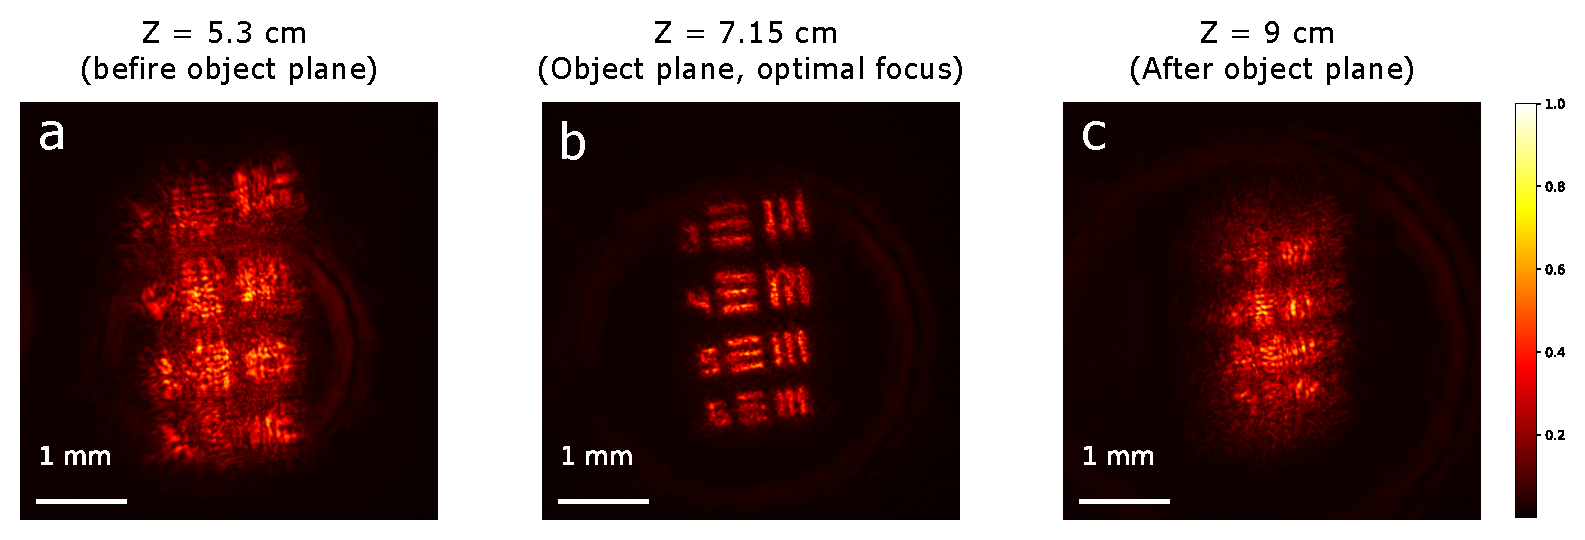
\includegraphics[width=0.93\textwidth]{figures/figure_S6.pdf}
            \renewcommand{\thefigure}{S6}
            \captionof{figure}{\footnotesize\textbf{Digital autofocus capability through numerical propagation of the reconstructed complex field.} The reconstructed field intensity is shown at three different propagation distances: \textbf{a} z = 5.3 cm (before the object plane), \textbf{b} z = 7.15 cm (at the object plane, where optimal focus is achieved), and \textbf{c} z = 9.0 cm (after the object plane). The sharp focus visible in panel \textbf{b} confirms the correct object plane location, demonstrating that precise knowledge of the object-diffuser distance is not required during data acquisition as optimal focus can be determined computationally during post-processing. Scale bars: 1 mm.}
            \label{fig_S6}
        \end{minipage}
    \end{quote}
\end{ourresponse}


        
\begin{enumerate}[label=\arabic*., resume]
\item \leavevmode
\end{enumerate}
\vspace{-1em}
\begin{solved_reviewercomment}
    I am not sure I understand how focussing the illumination on the scattering medium can reduce the fluctuations of \(E^{\text{ill}}_m\). Wouldn't it actually maximise them?    
\end{solved_reviewercomment}
\begin{ourresponse}
We thank the reviewer for this insightful question about an important aspect of our experimental design.

The reviewer's intuition that focusing on a scattering medium might maximize illumination fluctuations is valid for many scenarios. However, in our specific configuration, the opposite effect occurs due to a crucial relationship between the illumination spot size and the correlation length of the diffuser.

To address this question comprehensively, we have added a new section ("Effect of illumination spot size on coherent imaging through dynamic scattering") to the supplementary material with numerical simulations demonstrating this effect. For completeness, we reproduce the full section below:
\begin{quote}
    \section*{Effect of illumination spot size on coherent imaging through dynamic scattering}

In our coherent imaging configuration (Fig.~\ref{fig_5} of the main text), maintaining a constant illumination pattern at the object plane despite the dynamic scattering introduced by the rotating diffuser is crucial for successful application of our reconstruction algorithm. As expressed in Eq. 6-7 of the main text, our method requires that the illumination field $E_m^{ill}(\vec{r})$ remains effectively constant across different acquisitions for our method to work properly.

This requirement might appear contradictory, as one might expect that any illumination passing through a dynamic scatterer would inevitably result in varying illumination patterns. However, the key insight is that the relationship between the illumination spot size on the diffuser and the diffuser's correlation length determines whether the illumination at the object plane remains approximately constant between different diffuser realizations.

\begin{minipage}{\linewidth}
\centering
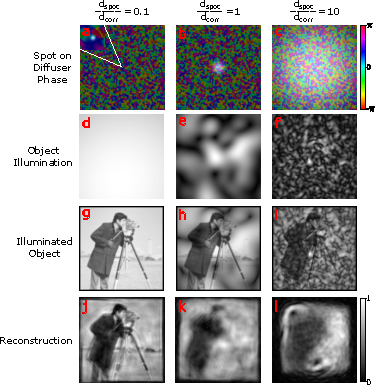
\includegraphics[width=0.93\textwidth]{figures/figure_S7.pdf}
\renewcommand{\thefigure}{S7}
\captionof{figure}{\footnotesize \textbf {Effect of illumination spot size on imaging through dynamic scattering.} 
Numerical simulations demonstrating how the ratio of illumination spot size ($d_{spot}$) to diffuser correlation length ($d_{corr}$) affects illumination at the object plane and reconstruction quality. Each column represents a different spot size ratio: $\frac{d_{spot}}{d_{corr}}=0.1$ (left), $\frac{d_{spot}}{d_{corr}}=1$ (middle), and $\frac{d_{spot}}{d_{corr}}=10$ (right). \textbf{a-c} Illumination phase pattern on the diffuser surface. The colorbar indicates phase values from $-\pi$ to $\pi$. The white inset in (a) shows the zoomed-in beam spot. \textbf{d-f} Resulting intensity patterns at the object plane after numerical propagation through the diffuser. The grayscale colorbar indicates normalized intensity. \textbf{g-i} Effective object (target object multiplied by the illumination pattern). \textbf{j-l} Reconstructed images after applying the I-CLASS algorithm. Note how a small spot size relative to the diffuser correlation length (left column) maintains relatively uniform illumination at the object plane, enabling high-quality reconstruction, while larger spot sizes (middle and right columns) create varying speckle patterns that degrade reconstruction quality.}
\label{fig_S7}
\end{minipage}

Fig.~\ref{fig_S7} demonstrates this principle through numerical simulation. The top row (Fig.~\ref{fig_S7}a-c) shows the phase pattern of the diffuser with the illumination spot superimposed for three cases: where the spot size is 0.1, 1, and 10 times the diffuser correlation length ($d_{\text{correlation}}$), respectively. The second row (Fig.~\ref{fig_S7}d-f) shows the resulting illumination intensity pattern at the object plane after the light has propagated through the diffuser, simulated using Fourier transform propagation.

When the illumination spot is much smaller than the diffuser correlation length (Fig.~\ref{fig_S7}a), it effectively samples only a single "phase patch" of the diffuser. As the diffuser rotates between realizations, this results in a relatively uniform illumination at the object plane that experiences only a global phase shift but maintains its spatial intensity pattern across different realizations. This consistency across different diffuser positions is crucial for our method to work properly. In other words, while the global phase of the illumination might change, its spatial distribution pattern remains effectively identical from one diffuser position to the next, satisfying our requirement for constant spatial illumination.

In contrast, when the illumination spot size is comparable to or larger than the diffuser correlation length (Fig.~\ref{fig_S7}c), the beam simultaneously samples multiple uncorrelated regions of the diffuser. This produces complex speckle patterns at the object plane that vary significantly between diffuser positions, creating a different illumination pattern for each diffuser realization. This variation violates our assumption of constant illumination in Eq. 6-7 of the main text.

The third row (Fig.~\ref{fig_S7}g-i) shows the effect of these illumination patterns on the effective object (the product of the object and the illumination), while the fourth row (Fig.~\ref{fig_S7}j-l) shows the reconstruction results. The reconstruction quality clearly degrades as the spot size increases relative to the diffuser correlation length, demonstrating the critical importance of maintaining consistent illumination across different diffuser realizations.

In our experimental implementation described in the main text, we carefully focused the beam to ensure a spot size smaller than the diffuser's correlation length ($\approx 70 \mu m$), thereby maintaining nearly constant spatial illumination patterns at the object plane across different realizations, with variations limited primarily to global phase shifts.
\end{quote}

\end{ourresponse}



\begin{enumerate}[label=\arabic*., resume]
\item \leavevmode
\end{enumerate}
\vspace{-1em}
\begin{solved_reviewercomment}
    I am slightly confused by the setup diagram in Fig.~\ref{fig_5}: The role of the polarizing beam splitter near the scattering medium is clear, as it allows to reject part of the unscattered light, thus maximizing the amount of useful signal, but the polarizing beam splitter closer to the camera seems to ensure that the signal and the reference have opposite polarizations, and thus can never interfere. Am I missing something, or is the diagram wrong?
\end{solved_reviewercomment}

\begin{ourresponse}
    We thank the reviewer for their careful examination of our experimental setup. The reviewer is correct - this was an error in our diagram. It should indeed be a non-polarizing beam splitter (BS), not a polarizing beam splitter (PBS). We have corrected this in the revised manuscript.
            
    \vspace{1em}
    \begin{minipage}{\linewidth}
        \centering
        \includegraphics[width=0.93\linewidth]{figures/figure_5.pdf}
        \renewcommand{\thefigure}{5}
        \captionof{figure}{\footnotesize\textbf{Experimental coherent reflection-imaging through dynamic scattering.} 
        \textbf{a} Experimental setup: A reflective target is illuminated through a dynamically rotating scattering diffuser. $M=180$ reflected light fields are holographically recorded in an off-axis holography configuration using a reference arm. %The illumination beam is focused to a tight spot on the diffuser surface such that the object illumination remains relatively constant while the diffuser is rotated.
        \textbf{b} Example of the recorded distorted fields after computational propagation to the object plane. \textbf{c} One example of the recorded field intensity after computational propagation to the object plane. 
        \textbf{d} Reconstructed object intensity at the object plane after applying the I-CLASS algorithm to compensate for scattering, revealing the details of the target. 
        \textbf{e} Complex-valued field amplitude PSFs (APSFs), estimated from the captured fields after effective deconvolution of the reconstructed object field. 
        \textbf{f} Reference intensity image of the object without the diffuser present. Scale bars, 1$mm$}
        \label{fig_5}
    \end{minipage}
\end{ourresponse}
        
\begin{enumerate}[label=\arabic*., resume]
\item \leavevmode
\end{enumerate}
\vspace{-1em}
\begin{solved_reviewercomment}
    The comparison between I-CLASS and the phase retrieval algorithms in the supplementary information seems weird. The fact that the phase retrieval is shown to never be able to reconstruct any image more complex than a few dots looks too bad to be true, and is at odds with my personal experience.
\end{solved_reviewercomment}

\begin{ourresponse}
    We thank the reviewer for raising this concern about the comparison between I-CLASS and phase retrieval-based methods.
    
    The comparison shown in the supplementary information is between I-CLASS and speckle correlation imaging that uses phase retrieval on an \textbf{estimated} autocorrelation, not standard phase retrieval on the true object spectrum.
    
    Standard phase retrieval operates directly on the exact power spectrum of an object, whereas speckle correlation imaging first requires estimating the object's autocorrelation from multiple scattered light patterns. The quality of this estimation affects the subsequent phase retrieval results.
    
    Following the reviewer's comment, we have revisited our speckle correlation implementations and improved the results by applying a more rigorous approach:
    
    For autocorrelation estimation:
    \begin{enumerate}
        \item Calculate the autocorrelation of each scattered frame
        \item Average all autocorrelations
        \item Divide the result by the autocorrelation of the mean of the images, which provides an estimate of the envelope of the PSF and subtract the envelope from all frames
        \item Subtract the minimum value to ensure non-negativity
        \item Apply appropriate windowing (square root of Tukey window for USAF target and fourth root of Tukey window for the cameraman)
    \end{enumerate}
    
    For phase retrieval, following Katz et al. (Nature Photonics, 2014):
    \begin{enumerate}
        \item Apply 300 iterations of HIO algorithm with decreasing beta parameters (from 2.0 to 1.2, decreasing by 0.2)
        \item Follow with 300 iterations of error reduction
        \item Implement object-specific constraints:
        \begin{itemize}
            \item  For the cameraman: real, positive, and non-negative constraints
            \item  For the USAF target: same constraints plus an additional finite square support
        \end{itemize}
    \end{enumerate}
    
    
    The updated figure now includes both our improved speckle correlation results and phase retrieval applied directly to the reference image for comparison. While our enhanced speckle correlation implementation shows better results than our original submission, I-CLASS still demonstrates better reconstruction quality, particularly for complex objects when the number of speckles in the PSF is limited, as is often the case in realistic experimental conditions.
    
    We have updated the supplementary section to reflect these improvements and provide a more comprehensive comparison.

                \begin{quote}
        \section*{Comparison with speckle-correlation phase-retrieval based reconstruction}

        We present a numerical comparison between our proposed I-CLASS method and the speckle correlation imaging of Katz et al. \cite{katz14}, which is, in essence, equivalent to running a phase-retrieval algorithm on the \textbf{estimated} object autocorrelation (that is, its power spectrum) as originally proposed by Labeyrie's stellar speckle interferometry \cite{labeyrie1970attainment}. 
        Both methods utilize similar experimental setups and image acquisition schemes, allowing for a direct performance evaluation. To perform this comparison, we focused on several numerically simulated isoplanatic imaging scenarios, demonstrating the superior performance of the matricial I-CLASS approach when reconstructing complex non-sparse natural target objects.
        
        For the speckle correlation reconstruction, we employ a rigorous approach to estimate the autocorrelation:
        \begin{enumerate}
            \item Calculate the autocorrelation of each scattered frame
            \item Average all autocorrelations
            \item Divide the result by the autocorrelation of the mean of the images, which provides an estimate of the envelope of the PSF and subtract the envelope from all frames
            \item Subtract the minimum value to ensure non-negativity
            \item Apply appropriate windowing (sqrt of Tukey window for USAF target and Tukey window $^{(1/4)}$ for the cameraman)
        \end{enumerate}
        
        For phase retrieval, following Katz et al. \cite{katz14}, we implement:
        \begin{enumerate}
            \item 300 iterations of HIO algorithm with decreasing beta parameters (from 2.0 to 1.2, decreasing by 0.2)
            \item 300 additional iterations of error reduction
            \item Object-specific constraints:
            \begin{itemize}
                \item For the cameraman: real, positive, and non-negative constraints
                \item For the USAF target: same constraints plus an additional finite square support
            \end{itemize}
        \end{enumerate}
        
        The results of this comparison are presented in Fig.~\ref{fig_S4}. The top row shows results for the Cameraman image, while the bottom row shows results for the USAF resolution target. For each test object, we display the widefield reference (Fig.~\ref{fig_S4}a,f), an example frame distorted by scattering (Fig.~\ref{fig_S4}b,g), the speckle correlation reconstruction (Fig.~\ref{fig_S4}c,h), the I-CLASS reconstruction (Fig.~\ref{fig_S4}d,i), and phase retrieval applied directly to the reference image (Fig.~\ref{fig_S4}e,j).
        
        While speckle correlation imaging produces recognizable reconstructions for both test objects, I-CLASS demonstrates higher reconstruction quality, particularly for the more complex Cameraman image.

        \begin{minipage}{\linewidth}
            \centering
            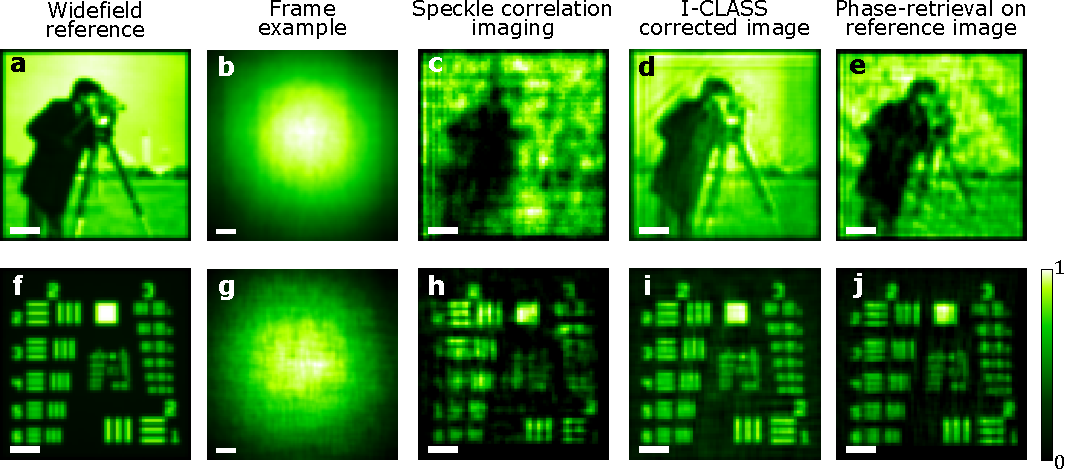
\includegraphics[width=0.93\linewidth]{figures/figure_S4.pdf}
                 \renewcommand{\thefigure}{S4}
            \captionof{figure}{\footnotesize\textbf{Numerical example imaging through dynamic scattering media.} 
            A comparison between I-CLASS and speckle correlation imaging for complex objects. \textbf{a,f} Numerically simulated target objects: the Cameraman image and USAF resolution target. \textbf{b,g} Example camera frames simulated under dynamic scattering. \textbf{c,h} Speckle correlation imaging reconstructions using the HIO algorithm (see parameters in text). \textbf{d,i} I-CLASS reconstructions showing higher fidelity to the original objects. \textbf{e,j} Phase retrieval applied directly to the reference images. Scale bar: 10 px.}
            \label{fig_S4}
        \end{minipage}
    \end{quote}

\end{ourresponse}

\begin{comment}
\hlyellow{\textbf{Note from Ori:}
the reason is that this is not standard phase-retrieval but phase-retrieval of speckle correlation imaging experiment: in a standard phase-retrieval the algorithm is run on the real power spectrum on the object (or equivalently the exact fourier-transform autocorrelation of the object) calculated directly from the object, whereas in our case the phase retrieval is run on an ESTIMATE of the object’s autocorrelation from the speckle correlation. In particular, for speckle correlation imaging to work, the speckled PSF autocorrelation has to resemble a highly-peaked delta-like function. This is the case ONLY when the PSF contains an extremely large number of speckles, since for a speckle field the autocorrelation peak to background ratio is proportional to the number of speckles contained in the PSF. This practically requires the captured scattered light image to contain a number of speckles that is considerably larger than the number of bright resolution cells in the target, which is not the case in our experiemnts and simulations]}
\hlred{Here we need to answer that it is correct that if you have the correct PSD of the object given some constraint there is a global minimum and you probably eventually converge there, however given non ideal estimation of the PSD (statistical speckle statistics error + noise) it works much worse, regrading statistical noise I would discuss the small PSF regime, and about the shot noise, I would cite Jerome's Optica paper about covariance noise, and claim that since we use the entire matrix and not just the diagonal we have better SNR}
\end{comment}

            
        \hl{example 1}
        
        \hlblue{example 2}
        
        \hlgreen{example 3}
        
        \hlred{example 4}
        
        \hlyellow{example 5}
        


\begin{comment}
    \textbf{This is the part copied from, and has to be added to the main manuscript:}
        \begin{quote}
            \subsection{CTR-CLASS}
            %Several key techniques for imaging through scattering layers within the 'memory-effect' region involve measuring the imaging system's transmission matrix. Recent advancements \cite{lee22,weinberg2024noninvasive} propose that, as the distortion caused by illumination does not hold any informative value, it's not necessary to measure the entire large matrix. Instead, one can effectively use a limited number ($M$) of random, uncorrelated illuminations for imaging, rather than analyzing the full matrix.
            Following the work of Lee et al. \cite{lee22}, we consider $m=1...M$ measured scattered light fields, $\vec{A}_m$ obtained under random uncorrelated illuminations, $\vec{S}_m$. By representing the optical transmission matrix from the illumination plane to the target plane as $\bm{P}_{ill}$, and the transmission matrix from the target plane to the camera plane by $\bm{P}_{det}$, each measured light field can be written as $\vec{A}_m = \bm{P}_{det}\bm{O} \bm{P}_{ill} \vec{S}_m$. The matrix $\bm{O}$ is the object transmission matrix. For a thin object, the matrix $\bm{O}$ is a diagonal matrix with the object transmission function along its diagonal.
            By incorporating the $M$ measurements, $\vec{A}_m$, as columns in a matrix $\bm{A}$, the entire measured dataset can be represented in a matrix form as:
            \begin{eqnarray}
            \bm{A} = \bm{P}_{det}\bm{O} \bm{P}_{ill} \bm{S}
            \label{eq:1}
            \end{eqnarray}
            where $\bm{S}$ is a matrix containing the input random patterns in its columns. By leveraging the fact that the illumination patterns are uncorrelated, i.e. $\bm{S}\bm{S}^\dagger = \bm{I + \epsilon}$ (where $\bm{I}$ is the identity matrix and $\bm{\epsilon}$ is the statistical noise matrix which diminishes as the number of realizations $M$ increases, eventually becoming negligible with a significant number of such uncorrelated illumination patterns), and the time-reversal symmetry of light propagation ($\bm{P}_{ill}\bm{P}_{ill}^{\dagger}=\bm{I}$), we can analyze the covariance matrix of $\bm{A}$: $\bm{R}=\bm{A}\bm{A}^{\dagger}$, as follows:
            \begin{eqnarray}
            \bm{R}=\bm{A}\bm{A}^\dagger = \bm{P}_{det}\bm{O}\bm{P}_{ill}\bm{S} \bm{S}^\dagger\bm{P}_{ill}^{\dagger} \bm{O}^\dagger \bm{P}^\dagger_{det} \nonumber \\ \approx \bm{P}_{det}\bm{O}_{eff} \bm{P}^\dagger_{det} = \bm{P}_{det}\bm{O}_{eff} (\bm{P}^{*}_{det})^T
            \label{eq:2}
            \end{eqnarray}
            
            where $\bm{O}_{eff} \equiv |\bm{O}|^2$ (see Supplementary S1 for further explanations). 
            
            Remarkably, as seen from Eq. 2, the covariance matrix $\bm{R}$ is mathematically analogous to the conventional reflection matrix from the camera plane to the object and back, when the target object is replaced by $\bm{O}_{eff}$. Hence, one can apply any conventional reflection-matrix analysis approach such as CLASS \cite{kang17,lee22} or distortion matrix \cite{badon2020distortion} on $\bm{R}$.
            
            We chose to apply the recently introduced memory-efficient version of the CTR-CLASS algorithm, whose code is publicly available \cite{weinberg2024noninvasive}, since it allows the application of the CLASS algorithm directly on high pixel-count holographic datasets without the need to explicitly compute the memory-demanding reflection matrix $\bm{R}$
 
        \end{quote}

        \textbf{This is the part copied from, and has to be added to the supplementary:}
        \begin{quote}
            \section{CTR-CLASS}

            The linear nature of a coherent imaging system and the wave equation makes choosing a basis consisting of independent illumination patterns possible. By writing the matrix of the system in this basis (the Green's function), we can fully describe the imaging process. Furthermore, if this matrix is pre-measured, one can obtain the output for any given illumination pattern by multiplying the matrix with the corresponding pattern \cite{popoff2010measuring}.
            For instance, one possible choice for the basis is the set of point-illuminations, which aligns with the description of the imaging system in real space ($\vec{r}$-basis), such that using controlled illumination field $\vec{E}_{in} (\vec{r})$ the output field ${\vec{E}_{out}}(\vec{r})$ can be described as:
            \begin{eqnarray}
            \vec{E}_{out} = \bm{R}_{sys}\vec{E}_{in}
            \label{eq:1}
            \end{eqnarray}
            Conceptually, we can decompose the system's matrix into a product of three distinct matrices, each corresponding to a distinct phase in the imaging process:
            
            \begin{eqnarray}
            \bm{R}_{sys} = \bm{P}_{det}\bm{O}\bm{P}_{ill}
            \label{eq:2}
            \end{eqnarray}
            The first matrix $\bm{P}_{ill}$ represents the propagation through the optical system of the input field to the object plane. The second matrix $\bm{O}$ characterizes the interaction with the object, where this matrix is modeled as a diagonal matrix for thin objects, with the object reflection function $O(\vec{r})$ on its diagonal. The third matrix $\bm{P}_{det}$ governs the propagation of back from the object plane through the optical system to the detection. 
            
            However, due to the very high number of modes in most common systems, measuring the reflection matrix can be daunting and time-consuming. In many practical imaging scenarios, such comprehensive measurements may be unnecessary for imaging within the optical memory effect. Recognizing this, the CTR framework \cite{lee22} presents an alternative approach that exploits the time-reversal symmetry of the illumination process for a phase-only distortion - which translates into the fact the matrix $\bm{P}_{ill}$, which represents the illumination step, is approximated as a unitary matrix $(\bm{P}_{ill}\bm{P}^\dagger_{ill} \approx \mathbf{I})$.
            Instead of measuring the reflection matrix $\bm{R}_{sys}$ in an orderly set of modes, such as the point illumination basis or plane waves basis (in k-space), it is suggested to illuminate a set of random, uncorrelated illumination patterns.
            
            The $M$ random illuminations used in the CTR methodology can be arranged in a matrix $\bm{S}$ in the $\vec{r}$-basis, where each illumination pattern corresponds to a matrix column. Due to their uncorrelated nature, the matrix \textbf{S} approximately satisfies the property $\bm{S} \bm{S}^\dagger = \mathbf{I} + \mathbf{\epsilon} \approx \mathbf{I}$, where $\bm{I}$ is the identity matrix and $\mathbf{\epsilon}$ represents the statistical noise matrix, which diminishes as the number of realizations $M$ increases and becomes negligible with a sufficient number of such realizations.
            
            
            
            
            One can order the $M$ measurements in the columns of 'measurement matrix' $\bm{A}$ which can be written by:
            \begin{eqnarray}
            \bm{A} = \bm{R}_{sys}\bm{S} = \bm{P}_{det}\bm{O}\bm{P}_{ill}\bm{S}
            \label{eq:3}
            \end{eqnarray}
            Then, rather than directly examining the reflection matrix $\bm{R}_{sys}$, the algorithm focuses on the matrix $\bm{R} \stackrel{\text{def}} = \bm{A}\bm{A}^\dagger$, which, from our analysis above can be written by:
            \begin{eqnarray}
            \bm{R}=\bm{A}\bm{A}^\dagger = \bm{P}_{det}\bm{O}\bm{P}_{ill}\bm{S} \bm{S}^\dagger\bm{P}_{ill}^\dagger \bm{O}^\dagger \bm{P}^\dagger_{det} \approx \bm{P}_{det}\bm{O}_{eff} \bm{P}^\dagger_{det} = \bm{P}_{det}\bm{O}_{eff} (\bm{P}^{*}_{det})^T
            \label{eq:4}
            \end{eqnarray}
            where $\bm{O}_{eff} \stackrel{\text{def}} = \bm{O}\bm{O}^\dagger$ and has $|{O}(\vec{r})|^2$ on its diagonal, as $\bm{O}$ is diagonal matrix as we consider thin objects.
            
            This matrix $\bm{R}$ has a similar structure to a full system reflection matrix in the real space ($\vec{r}$-basis), with the same illumination and detection transfer matrix up to phase conjugation.
            In the context of imaging through a scattering medium within the memory-effect regime, we can further model the detection transfer matrix $ \bm{P}_{det}$ as a convolution Toeplitz matrix that represents the distorted point spread function (PSF) any point on the object is convoluted with.
            
            The CTR-CLASS algorithm takes advantage of this unique structure of matrix $\bm{R}$ and estimates $\bm{P}_{det}$ and $\bm{O}_{eff}$ using the CLASS algorithm \cite{kang17}. This is achieved by iteratively leveraging the shifted inter-column correlations within $\bm{R}$.
            A recent improvement introduced a memory-efficient version of the CTR-CLASS algorithm, significantly reducing memory usage to $O(MN)$, where $N$ denotes the number of camera pixels \cite{weinberg2024noninvasive}. This advancement enables the application of the algorithm to megapixel-scale images without the need to explicitly compute $\bm{R}$, which is sized $O(N^2)$.
            It's important to note that while any matrix-based scattering compensation method could theoretically be applied given $\bm{R}$, in this work, we specifically utilize the CLASS algorithm.
            
            \newpage
            \section{CTR-CLASS correction in a conjugated plane}
            As described above, the matrix $\bm{R}$ can be looked at as a reflection matrix for a system:
            \begin{eqnarray}
            \bm{R} = \bm{P}_{det}\bm{O}_{eff} (\bm{P}^{*}_{det})^T
            \label{eq:5}
            \end{eqnarray}
            
            Where for an 'isoplanatic' patch where the distortion does not rely on object coordinates, the matrix $\bm{P}_{det}(\vec{r}_{diff},\vec{r}_{obj})$ describes a transfer matrix from each point on the detection scattering phase mask $\vec{r}_{diff}$ is transmitted towards the object plane with coordinates $\vec{r}_{obj}$. Hence, the effective field in the effective object plane is: $\vec{E}_{obj} = \bm{P}_{det}\vec{E}_{in}$. Assuming free-space configuration and that the distance $d$ between the object and the scattering layer is large enough to apply the Fresnel diffraction approximation, we can derive given an input field ${E}_{in}(x,y)$ the field at the object plane:
            \begin{eqnarray}
            {E}_{obj}(x,y)= \frac{e^{\frac{i2 \pi d}{\lambda}}}{i\lambda d} \iint {E}_{in}(x',y') 
            e^{\frac{-i\pi}{\lambda d} [ (x-x')^2+(y-y')^2 ] } dx'dy'
            \label{eq:6}
            \end{eqnarray}
            where $\lambda$ is the field wavelength. Thus, in a similar way to Choi et al. \cite{choi2022flexible}, each element of $\bm{R}(\vec{r}_{in},\vec{r}_{out})$ can be described as an input field of a point-illumination at $\vec{r}_{in}$ from the diffuser plane and point-detection $\vec{r}_{out}$ at the diffuser plane:
            \begin{eqnarray}
            {E}_{in}(x,y)= e^{-i\phi(x_{in},y_{in})}\delta(x-x_{in},y-y_{in})
            \label{eq:7}
            \end{eqnarray}
            Where $\phi(x_{in},y_{in})$ is the phase distortion of the effective phase-mask and the sign is conjugated from Eq.~\ref{eq:5}. Using Eq.~\ref{eq:7} we obtain:
            \begin{eqnarray}
            {E}_{obj}(x,y) \propto  e^{-i\phi(x_{in},y_{in})}
            e^{\frac{-i\pi}{\lambda d} [(x-x_{in})^2+(y-y_{in})^2 ]}
            \label{eq:8}
            \end{eqnarray}
            Upon reflection from the effective object $O_{eff}$, the detection transfer matrix is applied:
            \begin{align}
            & {E}_{out}(x_{out},y_{out}) = e^{i\phi(x_{out},y_{out})} \frac{e^{\frac{i2\pi d}{\lambda}}}{i\lambda d} \iint {E}_{obj}(x',y')O_{eff}(x',y') 
            e^{\frac{i\pi}{\lambda d} [ (x_{out}-x')^2+(y_{out}-y')^2 ] } dx'dy'  \nonumber &\\ 
            &\propto e^{i\phi(x_{out},y_{out})} \iint e^{\frac{-i\pi}{\lambda d} [(x'-x_{in})^2+(y'-y_{in})^2 ]} O_{eff}(x',y') 
            e^{\frac{i\pi}{\lambda d} [ (x_{out}-x')^2+(y_{out}-y')^2 ] } dx'dy'
             \nonumber &\\ 
            &= e^{i[\phi(x_{out},y_{out})-\phi(x_{in},y_{in})]}e^{\frac{i \pi}{\lambda d}(x^2_{out}+y^2_{out}-x^2_{in}-y^2_{in})} \iint O_{eff}(x',y')e^{-i\frac{2 \pi}{\lambda d}[(x'(x_{out}-x_{in})+y'(y_{out}-y_{in})]}dx'dy'\nonumber &\\ 
            &\equiv e^{i\phi_{eff}(x_{out},y_{out})}\tilde{O}_{eff}(\frac{x_{out}-x_{in}}{\lambda d},\frac{y_{out}-y_{in}}{\lambda d}) e^{-i\phi_{eff}(x_{in},y_{in})}&
            \label{eq:9}
            \end{align}
            
            Where $\phi_{eff}(x,y) \stackrel{\text{def}} = \phi(x,y) + \frac{\pi}{\lambda d}(x^2+y^2)$ and $\tilde{O}_{eff}(\nu_x,\nu_y)$ is the Fourier spectrum of ${O}_{eff}$, leading to a scaled ${O}_{eff}$ with a scaling factor of ${\lambda d}$. 
            
            So $\bm{R}(\vec{r}_{in},\vec{r}_{out})$ has a structure of a matrix similar to an isoplanatic imaging object beyond scattering layers system reflection matrix in the $\vec{k}$-basis. This matrix format aligns with the input requirements for the CLASS algorithm \cite{kang17,lee22}.

        \end{quote}
\end{comment}


\bibliographystyle{plain}
\bibliography{bib}

\end{document}


